\section{Performance testing}
To investigate whether or not the primitives provided were suitable for the task, three benchmarks have been implemented, designed to be as similar as possible to real world scenarios.

\subsection{Test setup}
All the tests were performed by placing the devices being tested on a flat table with no obstacles at a distance of roughly 1 meter.
The devices were connected to a power source and rebooted before each round of tests.
Every application other than the one performing the measurements was closed.
All of the devices used for testing were running a non-modified version of the operating system installed by the manufacturer.
Table \ref{table:devices-used} contains a list of the devices used, their brand and model along with the version of Android that was installed.


\begin{table}[h]
\centering
\caption{Devices used to test}
\label{table:devices-used}
\begin{tabular}{lllll}
\hline
Name          & Manufacturer      & Model name      & Android version           \\ \hline
Nexus 4       & Google            & Nexus 4         & Android 5.1.1             \\
Nexus 5       & Google            & Nexus 5         & Android 5.1.1             \\
Nexus 7       & Google            & Nexus 7         & Android 5.1.0             \\
OnePlus One 1 & OnePlus           & One             & CM 12.0S (Android 5.0.2)  \\
OnePlus One 2 & OnePlus           & One             & CM 12.0S (Android 5.0.2)  \\
Redmi         & Xiaomi            & Redmi 2         & Miui 6.0 (Android 4.4.2)  \\ 
\hline
\end{tabular}
\end{table}

\subsection{Throughput}
This test was designed to measure the transmission performance of Bluetooth in the context of a long lasting connection to a single other device such as the exchange of a picture or video.
The metric of interest was throughput, which is defined as the number of bytes transferred per second.

A single round of test worked by connecting two devices, a client and a server and performing 20 transfers using the same connection.
Each of the 20 transfers measured the time needed to send a test payload of 2000 kbytes from the server to the client.
The pseudo code for client and server is shown in Algorithm \ref{pseudo:tr_client} and \ref{pseudo:tr_server}.
When 20 transfers were completed the data collected was saved for further processing.

\begin{algorithm}
	\begin{algorithmic}[1]
  		\caption{client pseudocode}
  		\label{pseudo:tr_client}
		\State $socket \leftarrow connectToServer()$
		\State $results \leftarrow emptyList()$
		\For{$i=1$ to $20$}
		    \State $T_0 \leftarrow nanotime()$ \Comment current time in nanoseconds
			\State $data \leftarrow socket.read(2048000)$ 
			\State $T_1 \leftarrow nanotime()$
			\State $list.add(T_1 - T_0)$
		\EndFor
		\State \Return $results$
  	\end{algorithmic}
\end{algorithm}

\begin{algorithm}
	\begin{algorithmic}[1]
  		\caption{server pseudocode}
  		\label{pseudo:tr_server}
  		\State $socket \leftarrow serverSocket.accept()$
		\Repeat
		    \State $data \leftarrow randomByteArray(2048000)$
            \State $socket.write(data)$
		\Until{client closes the connection}
		\State \Return $results$
  	\end{algorithmic}
\end{algorithm}

In order to collect a meaningful amount of data the test was performed multiple times using different devices as client and server.
The devices used along with the number of measurements performed are shown in Table \ref{table:tr-measurements}.

\begin{figure}[h]
  \centering
  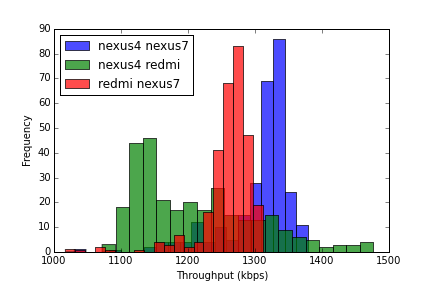
\includegraphics[width=1.0\textwidth]{application/img/tr-distribution.png}
  \caption{Distribution of throughput for each pair of devices tested.}
  \label{figure:tr-distribution}
\end{figure}

\begin{table}[ht]
\centering
\begin{tabular}{llll}
\hline
Client        & Server      & Number of rounds &  Failed  \\ \hline
Nexus 4       & Nexus 7     & 15               & 1        \\
Redmi         & Nexus 7     & 15               & 0        \\
Nexus 4       & Redmi       & 15               & 0        \\
\hline
\end{tabular}
\caption{Devices used to compute troughput and number of rounds}
\label{table:tr-measurements}
\end{table}

For each measurement $(T_0, T_1, N)$ collected, the throughput in $kbps$ was computed as 
\[\frac{N*8/1000}{T_1 - T_0}\]
where $N$ was the number of bytes, $T_0$ was the initial time and $T_1$ was the final time.

The distribution of throughput for each pair tested, is shown in Figure \ref{figure:tr-distribution}.

The average throughput, computed as the mean of all the values, was $1258 kpbs$ which is a value sufficient to send pictures taken from a modern smartphone in just a few seconds.


\subsection{Cost of connection setup}
In applications designed to allow people to communicate, the time a message takes to be delivered is a fundamental parameter.
The delivery time can be split in two parts: the setup of the Bluetooth connection and the transfer time for the message.
Analyzing the impact of the time required for the setup of the connection over the total time required for the delivery of the message is particularly important in the context of multi-hop communication systems, where each node has to hold (hence setup) a large amount of connections with other peers of the system.

The benchmark tested the connection setup cost and the time required to transfer messages of different sizes between two devices.
In order to make sure that the network wasn't loaded and the connection setup cost was being evaluated correctly only one device at a time could send messages.
At the beginning of the test, a token is created by the master. At most one device can hold the token at a certain time. This ensures that only one device at a time is allowed to send messages.
During a run of the test, the devices are organized in a circular ring, and every time a device receives the token it sends a message to the next device in the ring and takes some measures about connection time and transfer time. Then, it sends the token to the next device that will repeat the process.
The pseudo code for a peer in the ring is shown in Algorithm \ref{pseudo:ring_peer}.

\begin{algorithm}
	\begin{algorithmic}[1]
  		\caption{Ring peer pseudocode}
  		\label{pseudo:ring_peer}
  		\While {true}
		\State $socket \leftarrow serverSocket.accept()$
		\State $ping \leftarrow socket.read(payloadSize)$
		\State $socket.write(pong)$
		\State $token \leftarrow receiveToken()$
		\State $nextDevice \leftarrow nextPeer()$ \Comment next peer in ring
		\State $T_0 \leftarrow nanotime()$ \Comment current time in nanoseconds
		\State $newSocket \leftarrow nextDevice.connect()$
		\State $T_1 \leftarrow nanotime()$ 
		\State $newSocket.write(ping(randomByteArray(payloadSize)))$
		\State $pong \leftarrow socket.read()$
		\State $T_2 \leftarrow nanotime()$
		\State $token.times.add(T_0, T_1, T_2)$
		\State $socket.write(token)$
		\EndWhile
  	\end{algorithmic}
\end{algorithm}

The master is designated when the test starts and it is responsible for sending the first ping to the following device in the ring, in order to start the test.
It is responsibility of the master to stop the loop as well, when the token has traveled through the ring for a defined number of times.

\subsubsection{Test execution}
In order to be sure to collect a sufficient amount of data, the test was performed multiple times and with different configurations.
The test has been performed on 4 sets of devices, forming 4 different ring configurations.
For each of those ring configurations, the test has been executed a total of 40 times, 10 times for each payload size.
Before every test, all the devices have been rebooted.
A test was considered finished when the token passed through every peer in the ring 5 times.

In a portion of the tests that have been executed a problem has arisen, preventing the test from finishing successfully.
In those cases, the token would be blocked inside the ring mainly due to errors in the setup of the connection, preventing the test from continuing.
When this occurred, data collected up to that point was saved and the the test continued with the next run.
It is important to note that if a test consisting in $N$ token hops failed at the $n$th one, the remaining $N - n$ hops weren't completed and were accounted as failed transmissions.
However, this would be less of an issue in network topologies other than a ring, where the failure of a node would not necessarily impact the delivery of the message.

The correlation between rate of messages lost and configuration of the ring of devices is shown in Table \ref{table:failure_rate_ring_config}.
The correlation between failures and size of payload transmitted, on the other hand, is shown in Table \ref{table:failure_rate_payload_size}.

\begin{table}[ht]
\centering
\begin{tabular}{llll}
\hline
Devices                             & Master      & Total   &  Failed    \\ \hline
Nexus 5, Nexus 4, Nexus 7           & Nexus 5     & 600     & 342        \\
Nexus 4, Nexus 5, Nexus 7           & Nexus 4     & 600     & 114        \\
Nexus 4, Nexus 5, Nexus 7, Redmi    & Nexus 4     & 800     & 256        \\
Redmi, Nexus 5, Nexus 7, Nexus 4    & Redmi       & 800     & 296        \\
\hline
\end{tabular}
\caption{Rate of messages that went lost by configuration of ring of devices}
\label{table:failure_rate_ring_config}
\end{table}


\begin{table}[ht]
\centering
\begin{tabular}{llll}
\hline
Size of payload (bytes) & Total     & Failed    \\ \hline
512                     & 700       & 213       \\
1024                    & 700       & 310       \\
2048                    & 700       & 251       \\
4096                    & 700       & 234       \\
\hline
\end{tabular}
\caption{Rate of messages that were lost by size of the payload transmitted}
\label{table:failure_rate_payload_size}
\end{table}

\subsubsection{Results}
This test highlighted the impact that the time taken to setup a connection has on the total time needed to send a message between two devices.
The cost of connection setup becomes less significant when the same connection is preserved and used for a longer period of time (i.e. when the communication is performed between two devices only), since the connection setup will affect only the first communication.

\begin{figure}[ht!]
  \centering
  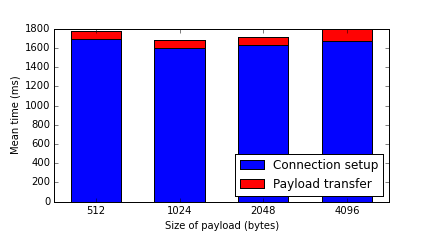
\includegraphics[width=1.0\textwidth]{application/img/setup_with_transfer.png}
  \caption{Average time for connection setup and message transmission for different sizes of payload}
  \label{figure:conn_vs_transfer}
\end{figure}

\begin{figure}[ht!]
  \centering
  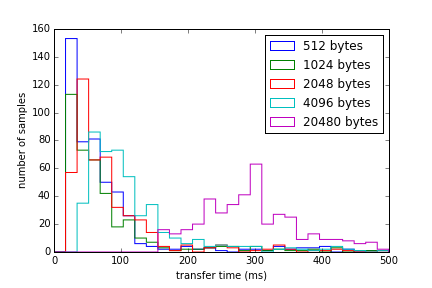
\includegraphics[width=1.0\textwidth]{application/img/transfer-time-distribution.png}
  \caption{Distribution of the time required to transfer a payload of different sizes}
  \label{figure:transfer_time_distribution}
\end{figure}

Fig. \ref{figure:conn_vs_transfer} shows the impact that the time taken to setup a connection has over the total time needed to send a message of different sizes.
For each set of measurements $(T_0, T_1, T_2, N)$, which represent respectively the time before the connection, after the connection and after the transmission of the message and the number of bytes transferred, the cost in time of connection setup was computed, for every payload size, as the mean of all the values $T_C = T_1 - T_0$.
The cost of transmission of the message was computed, for every payload size, as the mean of the values $T_T = T_2 - T_1$.
It is important to note that, given the small size of the payload sent during this test, measures taken about the transmission time are not to be considered fully accurate, in particular those involving the smallest payloads.

\begin{figure}[ht!]
  \centering
  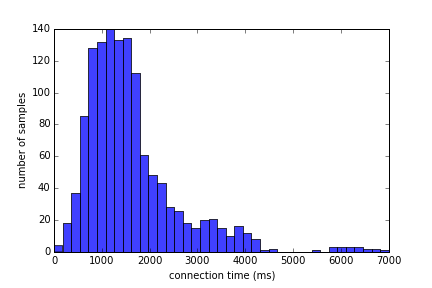
\includegraphics[width=1.0\textwidth]{application/img/setup_distribution.png}
  \caption{Distribution of time required to setup a connection between two devices. Three outliers are not shown in this figure due to their high value. More specifically, their values are 19105, 18956 and 7172 ms}
  \label{figure:conn_time_distribution}
\end{figure}

Fig \ref{figure:conn_time_distribution} shows the distribution of connection time observed during all the tests performed.
Size of payload was not considered because the time to setup the connection was measured before the transmission of any data. 
Data collected shows that the distribution of time required to open a connection does not change significantly using different pairs of devices.
Three outliers are not shown in the figure for representation purposes. Their values are 19105, 18956 and 7172 ms.
As can be seen, the vast majority of connections required a time between 1 and 2 seconds to setup.
However, a non negligible amount of connections required a considerably larger amount of time to setup.
Even though this behaviour was observed in a relatively small amount of samples, it should be taken into account when designing a system relying on the Bluetooth technology, particularly if this system is required to setup new connections frequently.
\subsection{Testing application}
All of the performance tests were executed by a standard Android application which was installed on all of the devices.
Since manually launching all of the test with different configurations would have been a very error prone task, the application embedded an HTTP server that allowed an operator to control all aspects of the test and retrieve the results at the end.
The HTTP server listened on port $38080$ until the application was closed.
This technique permitted manual testing when required but allowed a script to automatically perform various tests with different configurations automatically.

The HTTP server on the device exposed a few different endpoints, some of which were used to gather information about the device itself and others to run the tests.
For instance, a HTTP GET request on the \texttt{/mac} endpoint was used to get the Bluetooth MAC address and name for the device, information that was later used to run the tests.

When a HTTP request was used to run a test, it usually blocked until the test was complete. This allowed the device to return the results as part of the HTTP response in CSV (comma separated values) format.
When this was not possible, such as in the token test, the initial request returned a token which was then used on another endpoint to check the status and fetch the result of the computation.

For this test setup to work all of the devices had to be connected to the same Local Area Network and the IP addresses were used as input for the script. 

All of the code developed is available on Github \cite{test-code}.
\subsection{Problems encountered}
A variety of issues have contributed in making the development of the application more difficult.
Different devices have often difficulties communicating through Bluetooth, especially when running different versions of the operating system. This could be caused by small changes in Android's Bluetooth stack, or by issues unique to a specific model.
It is important to note that, starting with version 4.2 of the operating system, Android switched its Bluetooth stack from BlueZ, the linux Bluetooth stack, Bluedroid, which is developed by Broadcom. This could potentially be the cause of some of the issues encountered, since Bluedroid was immature when Google decided to include it in Android.

The issues experienced can be broadly divided into three categories: errors that interrupted an established communication, issues that prevented the setup of a connection and misuse of the API due to poor documentation.

The first type of error manifested itself as a \texttt{IOException: Broken Pipe} and was usually related to a race condition that caused a socket on either end of a connection to be erroneously closed.
The issue disappeared as soon as we fixed the application's code.

Errors while setting up a connection were a lot more frequent and, as far as we know, not caused by an error in the application.
They would always manifest themselves as \texttt{IOException: read failed, socket might closed or timeout, read ret: -1}.
After some research on developer communities it appears that this is a common issue with Bluetooth connections but nobody has been able to track down the root cause of it yet.
Some developers claimed that a fix involving java reflection solved this problem in their application and provided code for others to use.
Including the workaround in the code did not prove effective in our case.
This particular error is the cause of all the reported failures in the tests.

While we were unsuccessful in preventing the issue from happening we noticed some patterns in how the error manifested itself.
Performing a number of tests with a big enough pause (at least 60 seconds) between them seemed to lower the incidence of the problem.
Also the problem appeared a lot more frequently when more than two devices where involved in the communication, like in the token test.

Finally, the documentation provided on the Android website isn't very complete.
For instance, we discovered that we could not open more than one concurrent connection to the same remote device.
While this problem was easy to fix, the fact that such a surprising behavior is undocumented shows that Bluetooth is not yet a mature platform in the Android applications ecosystem.
